\documentclass[titlepage]{article}

\usepackage{fancyhdr}
\pagestyle{fancy}

\usepackage{xcolor}
\definecolor{Gray}{rgb}{0.5,0.5,0.5} % خاکستری

\usepackage[pdfborder={0 0 0}, bookmarks=true]{hyperref}
% آپشن اول بردر ها لینک را حذف میکند و باید دستی لینک ها را اندر لاین کرد

\usepackage{graphicx}
\graphicspath{ {./img/} }

\usepackage[most]{tcolorbox}

\usepackage{changepage}

\usepackage{listings}
\lstset{
  basicstyle=\ttfamily\small,           % فونت اصلی برای کد
  numbers=left,                         % شماره خطوط در سمت چپ
  numberstyle=\tiny\color{Gray},        % استایل شماره خطوط
  breaklines=true,                      % شکستن خطوط بلند
  breakatwhitespace=true,               % شکستن خطوط در محل فاصله‌ها
  showstringspaces=false,               % حذف فاصله‌های خاص در رشته‌ها
  tabsize=2,                            % اندازه تب
  captionpos=b,                         % موقعیت عنوان (بالا/پایین)
}

\usepackage{comment}

\begin{document}

\tcbset{
  inline/.style={
    colframe=gray,                     % رنگ قاب
    colback=gray!10,                   % رنگ پس‌زمینه
    fonttitle=\bfseries,               % استایل عنوان
    boxrule=0.4pt,                     % ضخامت قاب
    left=-1pt, right=-1pt,             % فاصله متن از چپ و راست
    top=0pt, bottom=0pt,               % فاصله متن از بالا و پایین
    height=10.9pt,                     % ارتفاع ثابت باکس
    valign=center,                     % تراز عمودی محتوا در باکس
    baseline=2.9pt,                    % تنظیم خط پایه باکس
    before=\vspace{0pt},               % فاصله قبل از باکس
    after=\vspace{0pt},                % فاصله بعد از باکس
    enhanced,                          % فعال‌سازی تنظیمات پیشرفته
    breakable,                         % اجازه شکستن خطوط
    fontupper=\ttfamily\small,         % تنظیم فونت محتوای داخل باکس
  },
}
\tcbset{
  codebox/.style={
    colframe=gray,                     % رنگ قاب
    colback=gray!10,                   % رنگ پس‌زمینه
    boxrule=0.4pt,                     % ضخامت قاب
    left=1pt, right=1pt,               % فاصله از چپ و راست
    top=-4pt, bottom=-4pt,             % فاصله از بالا و پایین
    valign=center,                     % تراز عمودی محتوا در باکس
    enhanced,                          % فعال‌سازی تنظیمات پیشرفته
    breakable,                         % اجازه شکستن خطوط
  },
}
\tcbset{
  picframe/.style={
    colframe=gray,                     % رنگ قاب
    colback=gray!10,                   % رنگ پس‌زمینه
    boxrule=0.4pt,                     % ضخامت قاب
    left=1pt, right=1pt,               % فاصله از چپ و راست
    top=1pt, bottom=1pt,               % فاصله از بالا و پایین
    valign=center,                     % تراز عمودی محتوا در باکس
    enhanced,                          % فعال‌سازی تنظیمات پیشرفته
    breakable,                         % اجازه شکستن خطوط
  },
}

\title{\textbf{Computer Workshop\\Final Assignment}}
\author{Dr. MalekiMajd}
\date{Amir Mohammad Davoodi\\Winter of 4031}
\maketitle

\fancyhead{}
\fancyhead[L]{Final Assignment}
\fancyhead[R]{Computer Workshop Course}
\fancyfoot{}
\fancyfoot[C]{Page \thepage}

\tableofcontents 

\pagebreak

\section{Git and GitHub}

\subsection{Repository Initialization and Commits}
\begin{enumerate}
\item \textbf{Create a GitHub Repository}  
\\First, I created a new repository on GitHub. This repository would contain my \LaTeX \hspace{0pt} source files and the configuration for the workflow.
\item \textbf{Clone the Repository Locally} 
\\To work on the repository locally, I cloned it to my computer using the following command:  
\begin{adjustwidth}{1cm}{1cm}
\begin{tcolorbox}[codebox]
\begin{lstlisting}[numbers=none]
  git clone <repo_link>
\end{lstlisting}
\end{tcolorbox}
\end{adjustwidth}
\item \textbf{Local Changes and Git Operations}
\\After that, I made my changes locally and in each step, I added and committed changes, and pushed them to my GitHub repository, with the following commands:
\begin{adjustwidth}{1cm}{1cm}
\begin{tcolorbox}[codebox]
\begin{lstlisting}[numbers=none]
  git commit -am "commit message"
\end{lstlisting}
\end{tcolorbox}
\end{adjustwidth}
\begin{adjustwidth}{1cm}{1cm}
\begin{tcolorbox}[codebox]
\begin{lstlisting}[numbers=none]  
  git push --all
\end{lstlisting}
\end{tcolorbox}
\end{adjustwidth}
\end{enumerate}

\subsection{GitHub Actions for \LaTeX \hspace{0pt} Compilation}
In my local repository, I created a GitHub Actions workflow file named \tcbox[inline]{main.yml} in the \tcbox[inline]{.github/workflows/} directory. This file automates the process of compiling the \LaTeX \hspace{0pt} document into a PDF and releasing it whenever a new tag is pushed. 
\vspace{5pt}
\\I set up the workflow file as follows:
\begin{tcolorbox}[codebox]
\begin{lstlisting}
name: Release Compiled PDF 
on:
  push:
    tags:
      - '*.*.*'

jobs:
  build_latex:
    permissions: write-all
    runs-on: ubuntu-latest
    steps:
      - name: Set up Git repository
        uses: actions/checkout@v2
      - name: Compile LaTeX document
        uses: xu-cheng/latex-action@v2
        with:
          root_file: main.tex

      - name: Create Release
        id: create_release
        uses: actions/create-release@v1
        env:
          GITHUB_TOKEN: ${{ secrets.GITHUB_TOKEN }}
        with:
          tag_name: ${{ github.ref }}
          release_name: Release ${{ github.ref }}
          draft: false
          prerelease: false

      - name: Upload Release Asset
        id: upload-release-asset 
        uses: actions/upload-release-asset@v1
        env:
          GITHUB_TOKEN: ${{ secrets.GITHUB_TOKEN }}
        with:
          upload_url: ${{ steps.create_release.outputs.upload_url }} 
          asset_path: ./main.pdf
          asset_name: main.pdf
          asset_content_type: pdf
\end{lstlisting}  
\end{tcolorbox}
\vspace{5pt}
\noindent Here's a breakdown of what each part does:
\begin{itemize}
\item \textbf{Workflow Trigger (on)}
\\ The workflow is triggered when a tag with a version number (in the format of \tcbox[inline]{*.*.*}, such as \tcbox[inline]{1.0.0}) is pushed to the repository.
\item \textbf{Job (build\_latex)}
\\ This job runs on an Ubuntu-based virtual machine (\tcbox[inline]{runs-on: ubuntu-latest}).
\item \textbf{Steps:}
\begin{itemize}
\item Set up Git repository: Uses the \tcbox[inline]{actions/checkout@v2} action to clone the repository so that the workflow can access the \LaTeX \hspace{0pt} files.
\item Compile \LaTeX \hspace{0pt} file: Uses the \tcbox[inline]{xu-cheng/latex-action@v2} action to compile the \LaTeX \hspace{0pt} document \tcbox[inline]{main.tex} into a PDF. This step produces a \tcbox[inline]{main.pdf} file.
\item Create Release: Uses the \tcbox[inline]{actions/create-release@v1} action to create a GitHub release with the tag name based on the version pushed (e.g., \tcbox[inline]{1.0.0}). It sets the release as non-draft and non-prerelease, and attaches a release name (e.g., Release \tcbox[inline]{1.0.0}).
\item Upload Release Asset: Uses the \tcbox[inline]{actions/upload-release-asset@v1} action to upload the compiled PDF \tcbox[inline]{main.pdf} as an asset to the release created in the previous step. This allows users to download the PDF from the release page.
\end{itemize}
\end{itemize}

\section{Exploration Tasks}

\subsection{Vim Advanced Features}
Below are three advanced features of Vim that not have been covered in class:
\begin{enumerate}
\item \textbf{Text Objects}
\\Text objects in Vim are used to select a specific region of text based on its structure. Instead of manually selecting text by character or line, text objects let you select entire blocks of text such as paragraphs, sentences, or words.
Examples:
\begin{itemize}
  \item \tcbox[inline]{ciw} Change inside a word (deletes the word and allows you to insert new text).
  \item \tcbox[inline]{dap} Delete a paragraph.
  \item \tcbox[inline]{yi'} Yank text inside single quotes (copy the text within single quotes).
\end{itemize}
Text objects significantly enhance the speed and precision of text manipulation without needing to rely on the arrow keys.
\item \textbf{Macros (Recording Commands)}
\\Vim macros allow you to record a sequence of commands and then replay them to automate repetitive tasks. Macros are particularly useful when performing the same sequence of actions on multiple lines or chunks of text.
How to Use:
\begin{enumerate}
  \item Start recording with \tcbox[inline]{q} followed by \tcbox[inline]{a} letter (e.g., \tcbox[inline]{qa} to record to the register a).
  \item Perform the desired actions.
  \item Stop recording with \tcbox[inline]{q}.
  \item Replay the macro with \tcbox[inline]{@a}.
  \item You can also repeat the macro multiple times with a number prefix (e.g., \tcbox[inline]{5@a} to run the macro 5 times).
\end{enumerate}
Macros are powerful tools for efficiency in Vim, especially for repetitive editing tasks.
\item \textbf{Split Windows and Tabs}
\\Vim allows you to split the editor window both horizontally and vertically. This is useful when you need to view multiple files at once or reference different parts of the same file without losing context.
How to Use:
\begin{itemize}
\item Horizontal split: \tcbox[inline]{:split} or \tcbox[inline]{:sp}.
\item Vertical split: \tcbox[inline]{:vsplit} or \tcbox[inline]{:vsp}.
\item Navigate between splits using \tcbox[inline]{Ctrl+w} followed by the direction key (\tcbox[inline]{h}, \tcbox[inline]{j}, \tcbox[inline]{k}, or \tcbox[inline]{l}).
\item You can also use tabs (\tcbox[inline]{:tabnew}) to work with multiple files in separate tabs.
\end{itemize}
These features help in multitasking, enhancing the workflow and organization within Vim.
\end{enumerate}

\subsection{Memory profiling}
\subsubsection{Memory Leak}
A memory leak occurs when a program allocates memory dynamically but fails to release it properly when it’s no longer needed. Over time, the leaked memory accumulates and can eventually lead to the program consuming all available memory, causing it to crash or slow down significantly.
\noindent Memory leaks typically happen when a program allocates memory but does not free it correctly. This can occur for several reasons:
\begin{itemize}
\item \textbf{Forgetting to free memory:} If a program allocates memory using \tcbox[inline]{malloc} or \tcbox[inline]{calloc} but does not call \tcbox[inline]{free} when done, the memory is never released.
\item \textbf{Losing the reference to dynamically allocated memory:} If you overwrite a pointer that points to dynamically allocated memory without freeing it first, you lose the reference to the memory, making it impossible to free.
\item \textbf{Not handling errors correctly:} If an error occurs after memory allocation, and the program exits without releasing allocated memory, it results in a memory leak.
\end{itemize}
\subsubsection{Memory profilers}
\textit{Valgrind} is a programming tool used for memory debugging, memory leak detection, and profiling. It helps developers find memory-related bugs in their programs by detecting issues like memory leaks, uninitialized memory access, and improper memory deallocation.
\\\\\textbf{Purpose of Valgrind:}
\begin{itemize}
\item Detect memory leaks and memory corruption.
\item Check if memory is being accessed before it is initialized or after it has been freed.
\item Profile memory usage to detect areas where memory consumption is excessive.
\end{itemize}
\textbf{How Valgrind Helps with Memory Leaks:}
When you run your program through \textit{Valgrind}, it tracks all memory allocations and deallocations. If any memory is allocated and not freed before the program terminates, \textit{Valgrind} will report it as a memory leak.
\\To use \textit{Valgrind}, you should compile your C program with debugging information (-g flag) and run it under \textit{Valgrind} using:
\begin{adjustwidth}{1cm}{1cm}
\begin{tcolorbox}[codebox]
\begin{lstlisting}[numbers=none]  
valgrind --leak-check=full ./your_program.exe
\end{lstlisting}
\end{tcolorbox}
\end{adjustwidth}
This command checks for memory leaks and provides detailed information about where memory was allocated and not freed.
\\\textit{Valgrind} Example Output:
\begin{tcolorbox}[codebox]
\begin{lstlisting}
==1234== 1 bytes in 1 blocks are definitely lost in loss record 1 of 1
==1234==    at 0x4005F1: create_memory_leak (memory_leak.c:6)
==1234==    by 0x40061D: main (memory_leak.c:9)
\end{lstlisting}
\end{tcolorbox}
\noindent In this output, \textit{Valgrind} reports that one byte of memory was leaked at the location \tcbox[inline]{create\_memory\_leak} function, and provides the file and line number where the allocation occurred.
\\\\After finding leak you should make sure to make the following modifications to your code:
\begin{itemize}
\item Free dynamically allocated memory using \tcbox[inline]{free()} in C or \tcbox[inline]{delete} in C++.
\item Avoid accessing memory after it has been freed.
\item Initialize variables before use.
\end{itemize}

\subsection{GNU/Linux Bash Scripting}
\subsubsection{fzf}
Fuzzy searching is a technique that finds approximate matches to a given search query instead of requiring an exact match. It allows users to locate information even if they mistype words or use partial input by considering possible variations, omissions, or substitutions in the search string.
\\This technique is commonly used in search engines, spell checkers, and command-line tools like \textit{fzf}.
\vspace{8pt}
\\What does \tcbox[inline]{ls | fzf} do?
\begin{itemize}
\item \tcbox[inline]{ls} lists the files and directories in the current directory.
\item The output of \tcbox[inline]{ls} is then piped (\tcbox[inline]{|}) into \tcbox[inline]{fzf}, which provides an interactive interface to filter and select items using fuzzy searching.
\item You can type part of a filename, and \textit{fzf} will dynamically narrow down the list based on your input. Once you select an item and press Enter, the selected filename is returned to the terminal.
\end{itemize}
\subsubsection{Using fzf to find your favorite PDF}
\begin{enumerate}
\item To find all files with the \tcbox[inline]{.PDF} extension (case-insensitive), use the \tcbox[inline]{fd} command as follows:
\begin{adjustwidth}{1cm}{1cm}
\begin{tcolorbox}[codebox]
\begin{lstlisting}[numbers=none]
fd -e pdf
\end{lstlisting}
\end{tcolorbox}
\end{adjustwidth}
Explanation:
\begin{itemize}
\item \tcbox[inline]{fd}: A fast and user-friendly alternative to find.
\item \tcbox[inline]{-e pdf}: Searches for files with the extension .pdf (case-insensitive by default).
\end{itemize}
If you want to search case-sensitively, use \tcbox[inline]{-e PDF}.
\item Command to select a PDF using \textit{fzf}:
\begin{adjustwidth}{1cm}{1cm}
\begin{tcolorbox}[codebox]
\begin{lstlisting}[numbers=none]
fd -e pdf | fzf
\end{lstlisting}
\end{tcolorbox}
\end{adjustwidth}
Explanation:
\begin{itemize}
\item The pipe operator (\tcbox[inline]{|}) takes the output from the \tcbox[inline]{fd} command (list of found PDF files) and sends it as input to the next command (\tcbox[inline]{fzf}).
\item \textit{fzf} provides an interactive interface where you can:
\begin{itemize}
\item Start typing to filter the list dynamically.
\item Use arrow keys to navigate through the filtered results.
\item Press Enter to select a file, which will then be printed to the terminal.
\end{itemize}
\end{itemize}
\end{enumerate}
\subsubsection{Opening the file using Zathura}
To open the selected PDF file using \textit{Zathura}, you can use the following command:
\begin{adjustwidth}{1cm}{1cm}
\begin{tcolorbox}[codebox]
\begin{lstlisting}[numbers=none]
zathura "$(fd -e pdf | fzf)"
\end{lstlisting}
\end{tcolorbox}
\end{adjustwidth}
Explanation:
\begin{itemize}
\item \tcbox[inline]{fd -e pdf | fzf} is a way to interactively search for and select PDF files in a directory using two command-line tools: \tcbox[inline]{fd} and \tcbox[inline]{fzf} with piping.
\item \tcbox[inline]{\$(command)} The \tcbox[inline]{\$(...)} syntax captures the output of the command inside it and substitutes it as an argument to \tcbox[inline]{zathura}.
In this case, after selecting a PDF with \textit{fzf}, the full path to the file is passed to \textit{zathura} for opening.
\item \textit{Zathura} is a lightweight, keyboard-driven PDF viewer designed for minimalism and efficiency.
\end{itemize}

\section{Git and FOSS}

\subsection{README.md}
In the README, I provided an overview of the repository's purpose, which is to write assignment answers using \LaTeX \hspace{0pt} and automate the PDF generation process via GitHub Actions whenever a new tag and release are created. It outlines the repository structure, explaining the key directories such as \tcbox[inline]{/} for \LaTeX \hspace{0pt} file and readme file, \tcbox[inline]{/img/} for image assets used for \LaTeX \hspace{0pt} source file, and \tcbox[inline]{/.github/workflows/} for automation scripts. It also details the workflow steps for including writing answers, pushing changes, and triggering the GitHub Actions workflow to compile and upload the PDF and how to use the repository. Additionally, I included a list of tools I used for local compilation, and a section for acknowledgments. I tried to write The README as a comprehensive guide to understanding and utilizing the repository effectively.

\subsection{Issues}
You can see the issue that I submited in \href{https://github.com/MiliAxe/CW-Final}{\underline{this GitHub repository}} in below. 
\begin{tcolorbox}[picframe]
\centering
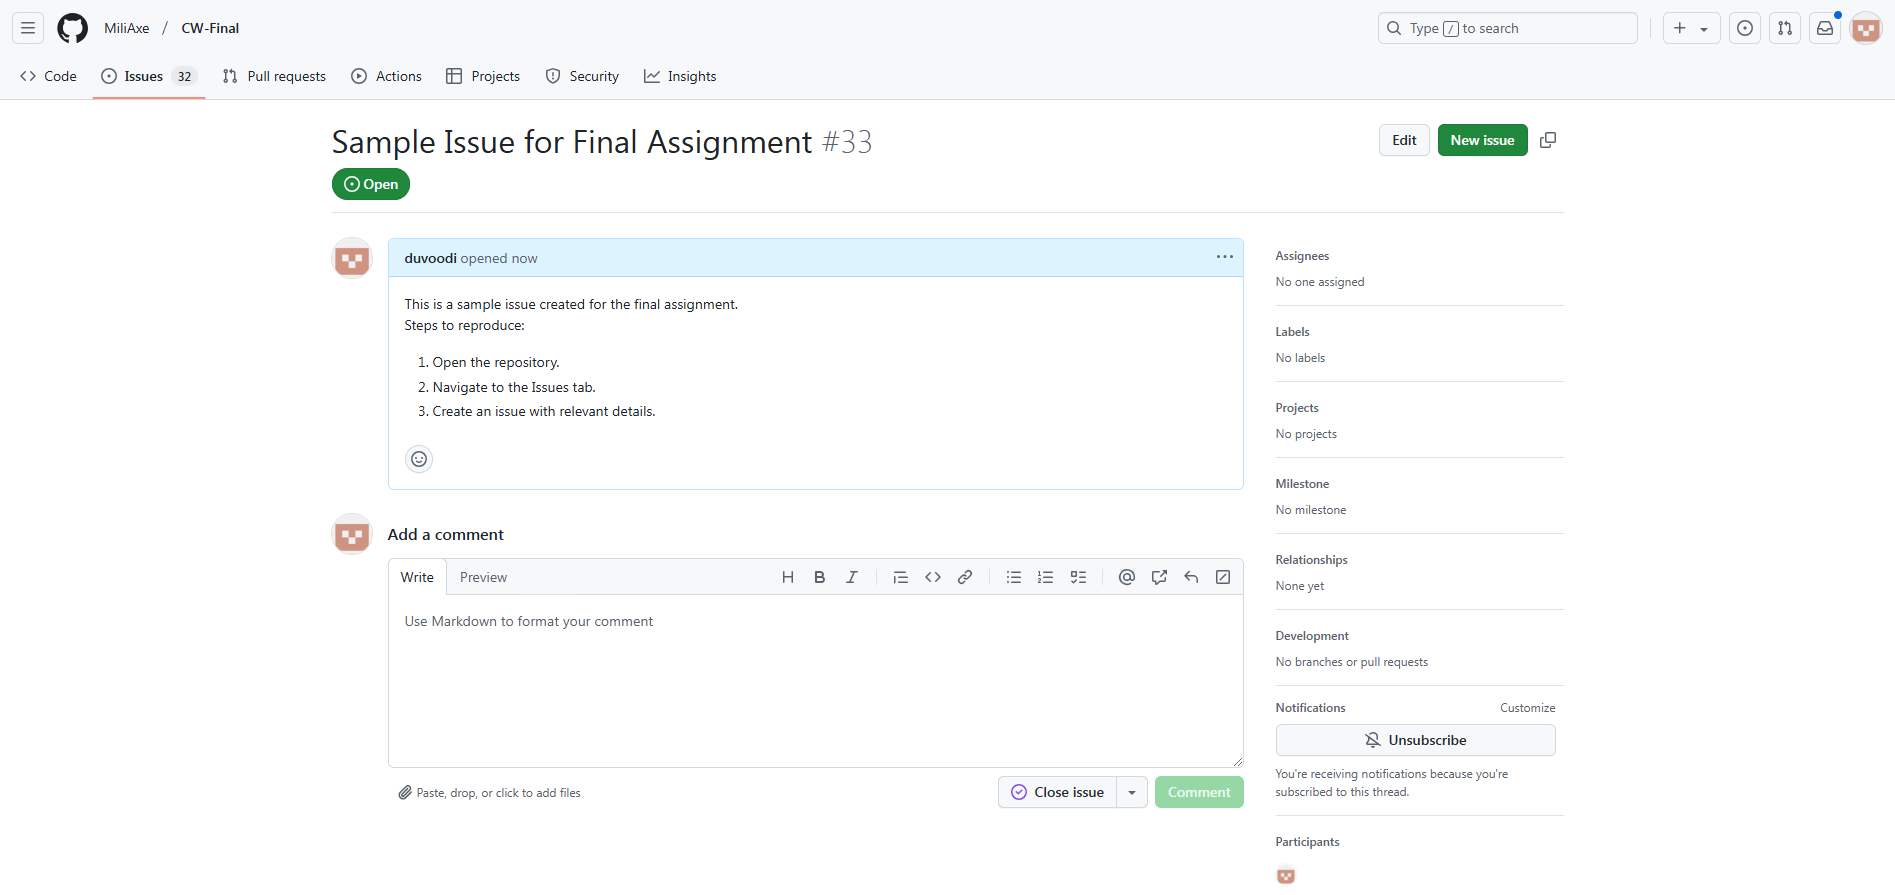
\includegraphics[width=\linewidth]{IssueScreenshot.png}
\end{tcolorbox}
\noindent Here is the link to this issue:
\\\url{https://github.com/MiliAxe/CW-Final/issues/33}

\subsection{FOSS contribution}
\textbf{Yes, I see myself contributing to FOSS projects in the future.}
\\Contributing to Free and Open Source Software (FOSS) projects is a great way to improve coding skills, collaborate with a global community, and give back to the tech ecosystem.  
\newpage
\textbf{My Areas of Interest for Contribution:}
\begin{enumerate}
\item \textbf{Developer Tools \& Automation:}  
\\These projects focus on improving development workflows and automation, making them ideal for developers who enjoy scripting and tooling. Tools that help streamline development workflows, such as CLI utilities, linters, and automation frameworks.  
\\Examples: 
\begin{itemize}
  \item \href{https://github.com/ohmyzsh/ohmyzsh}{\underline{OhMyZsh}}: A framework for managing Zsh configurations. Beginners can contribute by adding plugins, improving themes, or enhancing documentation.
  \item \href{https://github.com/Homebrew/brew}{\underline{Homebrew}}: A package manager for macOS and Linux. New contributors can help by improving formulae (package definitions), writing documentation, or fixing minor issues.
  \item \href{https://github.com/junegunn/fzf}{\underline{fzf}}: A fast command-line fuzzy finder written in Go. Contributions can include documentation improvements, creating tutorials, or fixing small bugs.
\end{itemize}
\item \textbf{Documentation \& Educational Projects:}
\\Improving documentation for beginner-friendly projects to help new contributors onboard easily.  
\\Examples:
\begin{itemize}
  \item \href{https://github.com/freeCodeCamp/freeCodeCamp}{\underline{freeCodeCamp}}: A platform for learning coding through hands-on projects. Beginners can contribute by improving existing learning materials or helping translate content.
  \item \href{https://github.com/TheOdinProject}{\underline{The Odin Project}}: A full-stack web development curriculum. Contributions include writing tutorials, reviewing lesson plans, and helping new learners in the community.
  \item \href{https://github.com/mdn/content}{\underline{MDN Web Docs}}: A comprehensive resource for web documentation. You can contribute by writing and editing documentation related to HTML, CSS, and JavaScript.
\end{itemize}
\item \textbf{Machine Learning \& Data Science:}
\\Open-source libraries that provide tools for AI/ML development.  
\\Examples:
\begin{itemize}
  \item \href{https://github.com/tensorflow/tensorflow}{\underline{TensorFlow}}: An open-source ML framework. Beginners can contribute by writing documentation, reporting issues, and adding simple tutorials.
  \item \href{https://github.com/scikit-learn/scikit-learn}{\underline{scikit-learn}}: A popular Python library for machine learning. You can contribute by improving examples, writing tests, or working on beginner-friendly issues.
  \item \href{https://github.com/fastai/fastai}{\underline{fastai}}: A library for deep learning based on PyTorch, with opportunities to contribute to code examples, tutorials, and library improvements.
\end{itemize} 
\item \textbf{Cybersecurity \& Privacy Tools:} 
\\Enhancing open-source security tools to help individuals and organizations secure their systems.  
\\Examples: 
\begin{itemize}
  \item \href{https://github.com/zaproxy/zaproxy}{\underline{OWASP ZAP}}: A security scanner for web applications. Beginners can help by improving documentation and reporting vulnerabilities.
  \item \href{https://github.com/bitwarden/clients}{\underline{Bitwarden}}: A password manager that welcomes contributors to its client applications and documentation.
  \item \href{https://github.com/letsencrypt/boulder}{\underline{Let's Encrypt}}: An open certificate authority. Contributions include improving documentation, writing automation scripts, and fixing minor bugs.
\end{itemize} 
\textbf{Reasons for Interest in FOSS Contributions:}  
\begin{itemize}
  \item \textbf{Skill Improvement:} Gain hands-on experience with real-world projects.
  \item \textbf{Networking:} Connect with like-minded developers globally.
  \item \textbf{Giving Back:} Contribute to the tools and platforms I benefit from daily.
  \item \textbf{Portfolio Building:} Display contributions for career opportunities.
\end{itemize}
Overall, FOSS contributions provide a fulfilling way to learn, collaborate, and impact the tech community positively.
\end{enumerate}

\end{document}